\label{tag:LTI}
\subsection{LTIについて}
LTI(Learning Tools IterOperability)とは、IMS Global Learning Consortium(以下、IMSと呼ぶ)が、異なるプラットフォーム間(異なるLMS上)における学習支援ツールの相互運用を可能とする技術に関する企画を策定し、標準化した規格のことである。LTIに準拠することの具体的なイメージとして、次のようなケースを想定することができる。先代の研究によりできたNSFをツール・プロバイダとし、異なるプラットフォーム間から利用するケース。(画像は後日作ってはります)\\
\subsection{LTIの基本的な用語について}
Tool Provider(ツール・プロバイダ)\\
Tool Provider(ツール・プロバイダ)とは、外部ツールや外部コンテンツのことでありツールを提供する側である、本研究ではNSFがツール・プロバイダにあたる。\\
Tool Consumer(ツール・コンシューマ)\\
Tool Consumer(ツール・コンシューマ)とは、ツール・プロバイダを使用するLMSのことである。LTIに準拠したLMSは例として、Canvas,Moodle,Sakai,blackbordなどがある。本研究ではMoodle、Canvasを使用した。\\
\subsection{LTI使用方法}
LMS上でTool Provider(ツール・プロバイダ)を使用するには、各LMS上で外部ツールの設定を変更する必要がある。例として、moodleでの使用方法を説明する。\\
moodleでは外部ツール設定より図\ref{fig:moodle config}参照、ツール名、ツールURL、コンシューマキー、秘密鍵の設定をする必要がある。これらの設定を得て、moodleからTool Provider(ツール・プロパイダ)を利用することが可能となる。\\
\begin{figure}[htbp]
  \begin{center}
    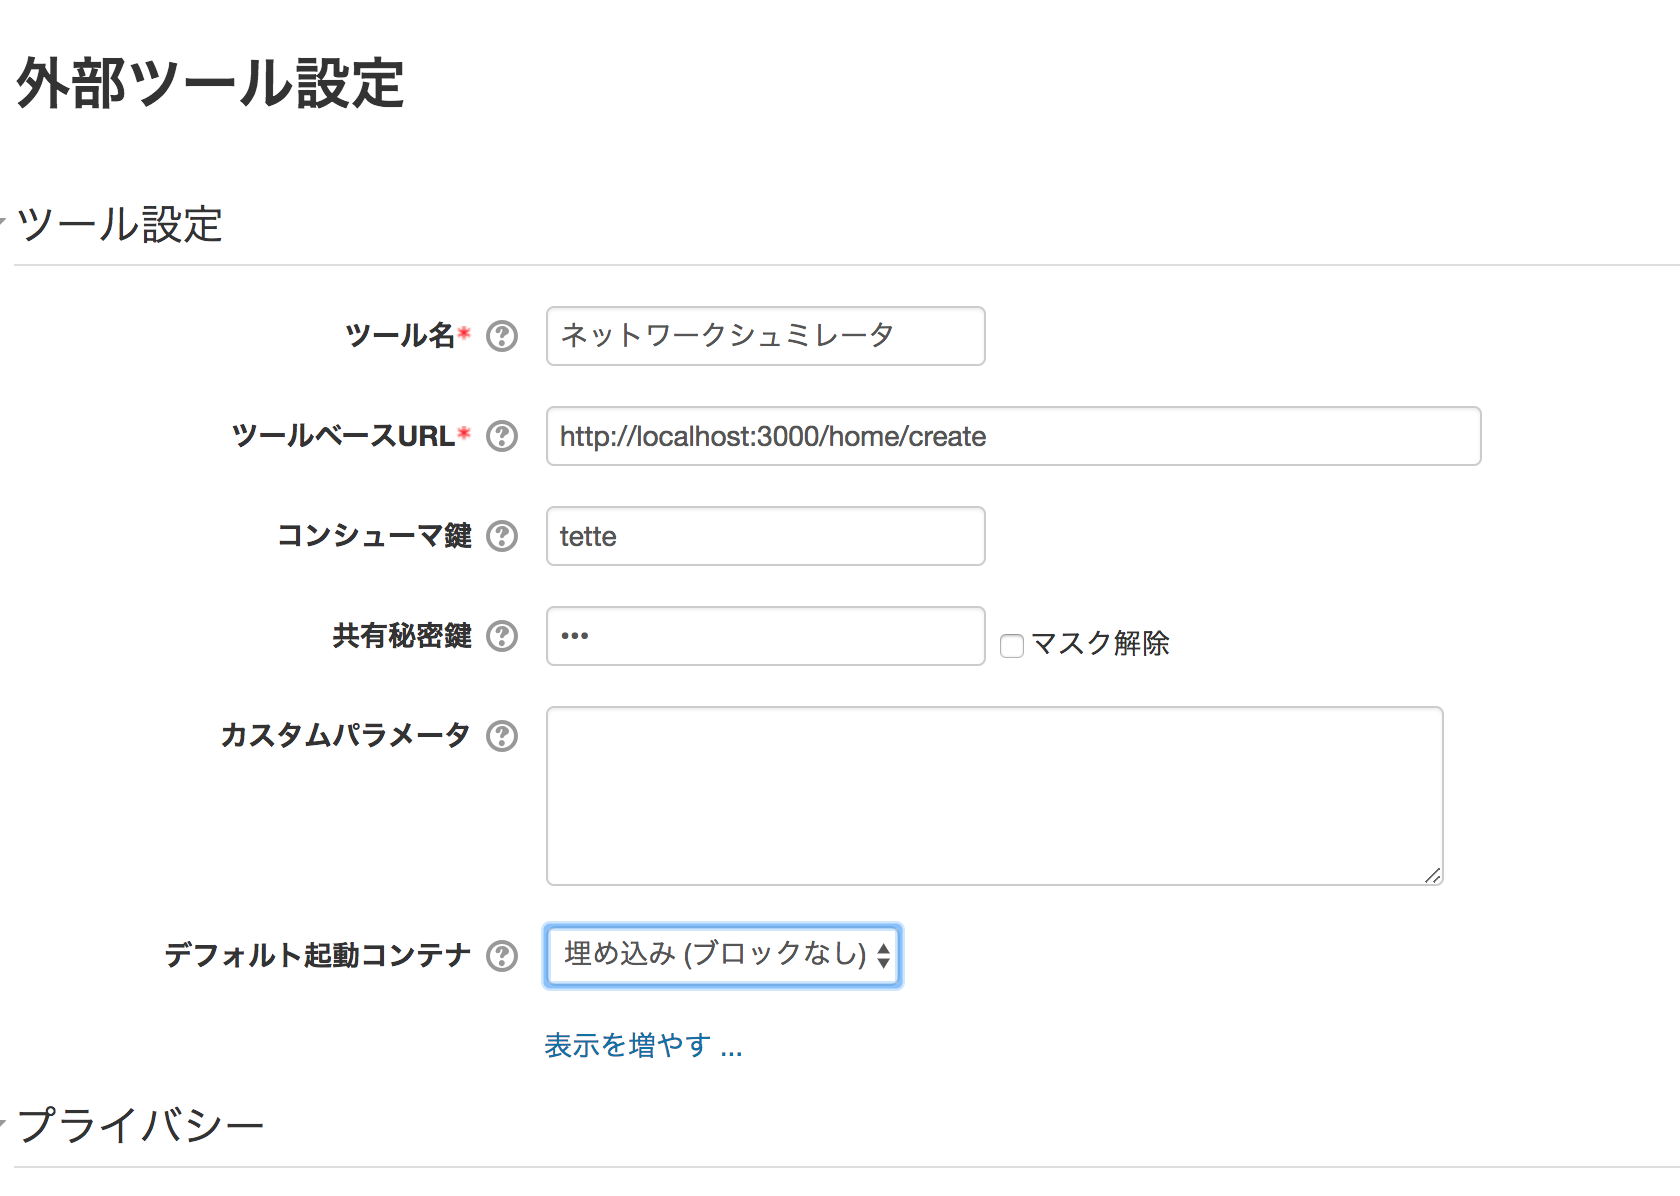
\includegraphics[clip,width=12.0cm,height=8.0cm]{img/moodleSet.png}
    \caption{moodle 外部ツール設定画面}
    \label{fig:moodle config}
  \end{center}
\end{figure}

\begin{figure}[htbp]
  \begin{center}
    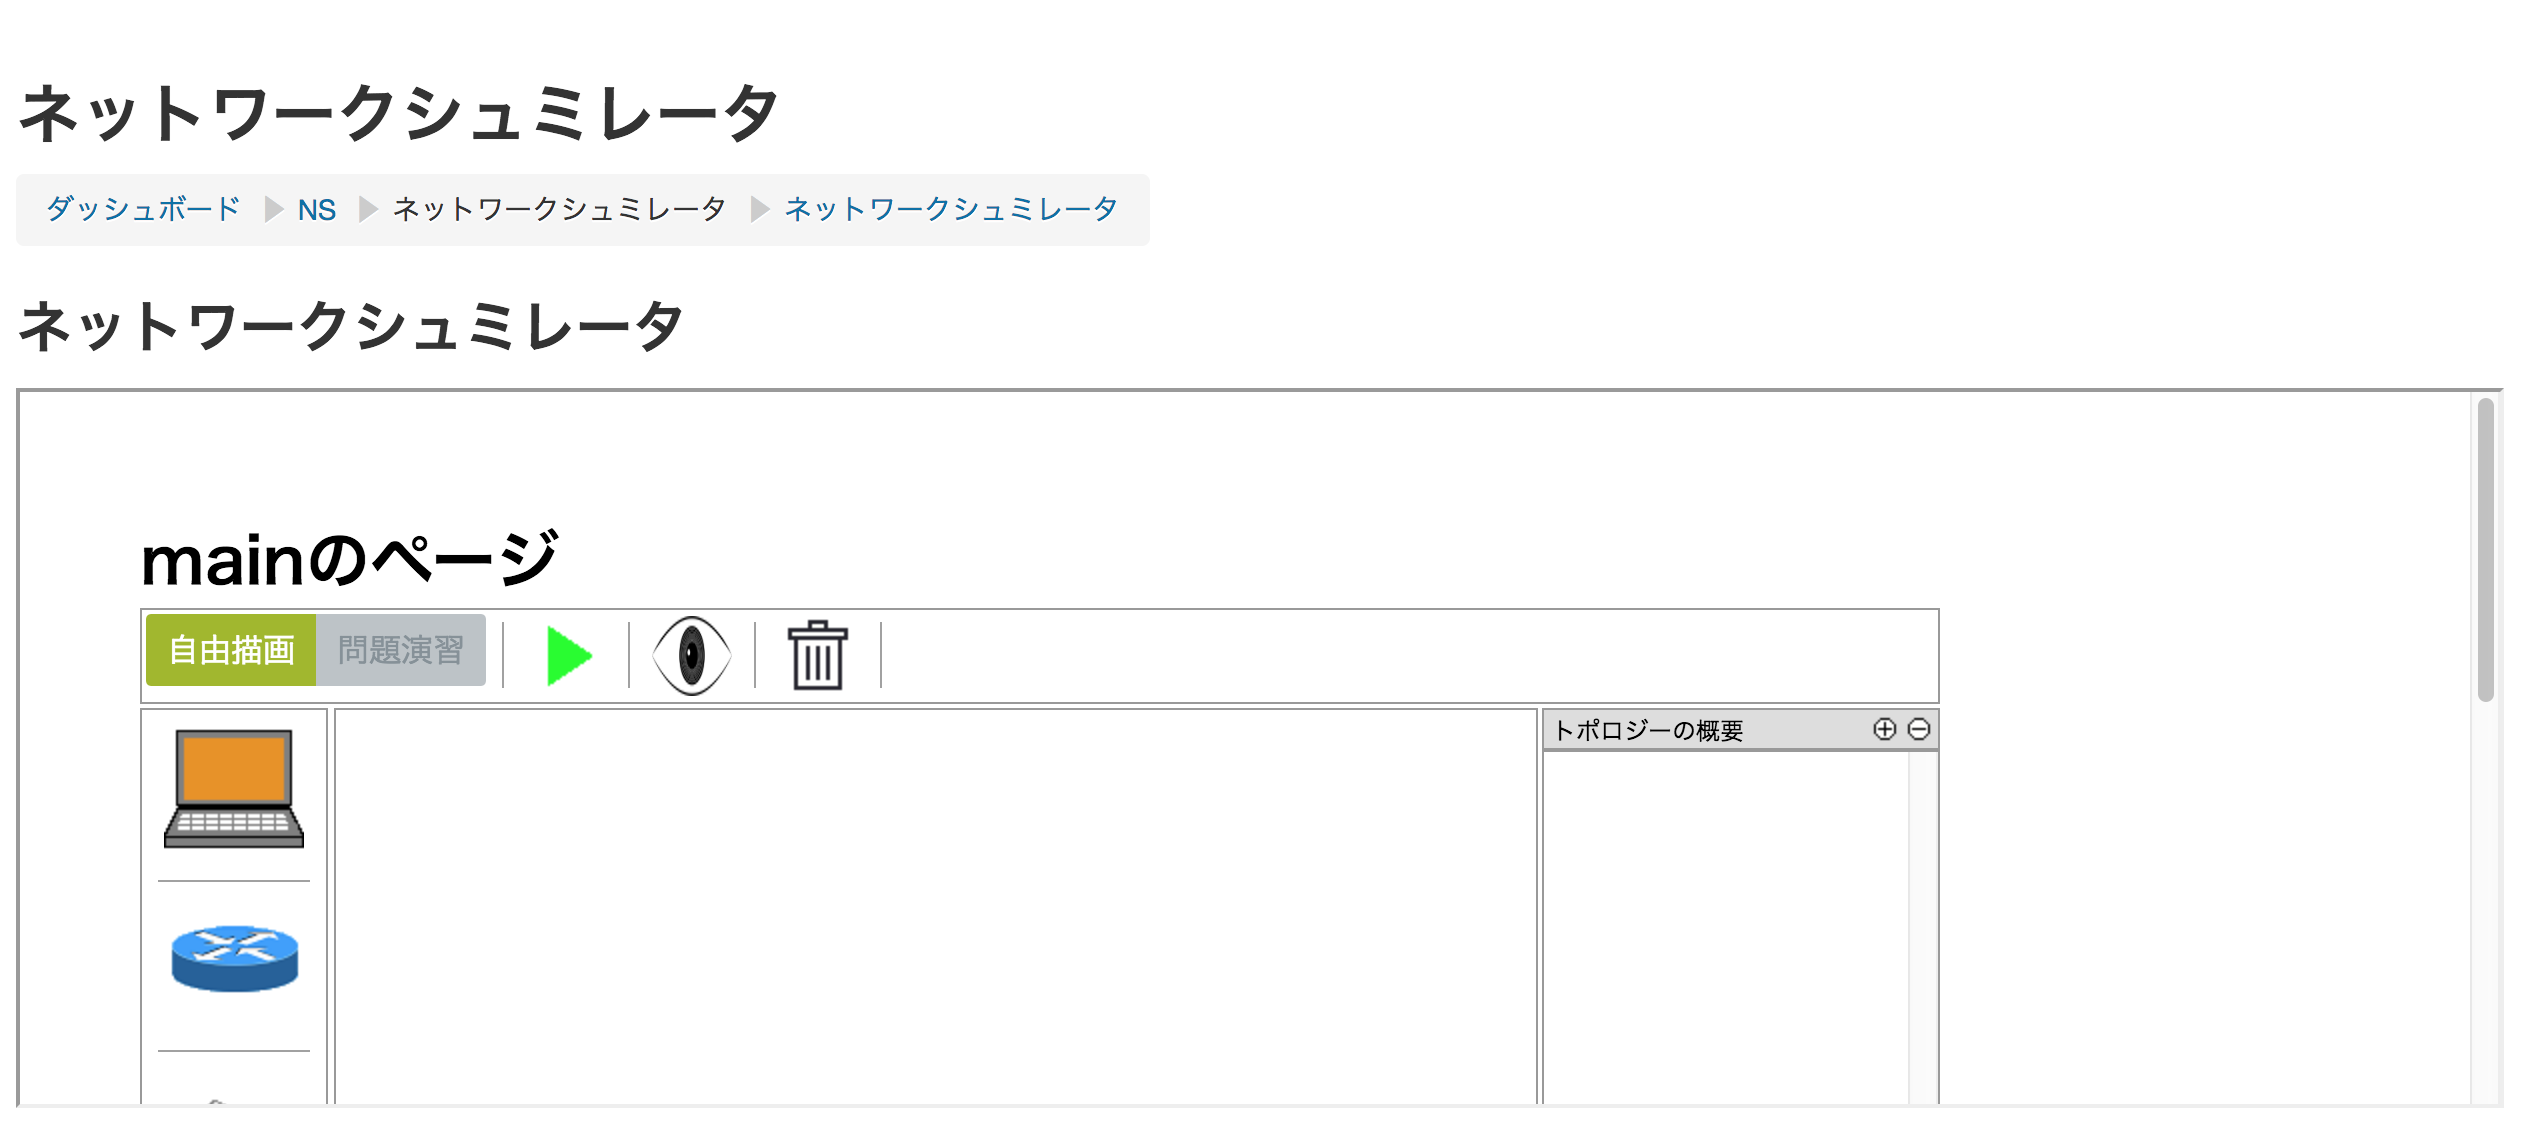
\includegraphics[clip,width=12.0cm,height=8.0cm]{img/LTIstart.png}
    \caption{moodle 外部ツール起動}
    \label{fig:moodle kidou}
  \end{center}
\end{figure}
また、ツール・プロバイダとツール・コンシューマとの間では、OAuthを用いて認証を行っている。\\
\subsection{OAuth}
OAuth(オーオース)とは、SNSやWebサービス間で「アクセス権限の認可」を行うためのプロトコルである。これにより、外部ツールへアクセスする際、ユーザIDとパスワードによる認証を行わずに外部ツールへのアクセスを行うことを可能にしている。また、OAuthには1.0と2.0が存在しているが、本研究ではLTI1.0の実装にあたりOAuth1.0を使用している。
\subsection{OAuth1.0実装手順}
OAuth1.0実装にあたり、OAuth signatureを作成する関数をRubyで自作した。\\
OAuth signatereの作成手順を以下に示す。\\
1.「キー」を作成\\
2.「データ」の作成\\
3.「キー」と「データ」用いてsignatureを作成aaa\\
\subsubsection{キーの作成}
「oauth\_consumer\_secret」、「oauth\_token\_secret」をURLエンコードし、&で繋げれば完成。\\
本研究では「oauth\_consumer\_secret」を設定し、「oauth\_token\_secret」は存在させなかった。また、各々をCGI.escapeによりURLエンコードし、「oauth token secret」を空白とし、&のみを繋げてKeyを作成した。
\subsubsection{データの作成}
1.パラメータをアルファベット順に並べ、キー=値...の形で並べた上で,URLエンコードする。\\
2.リクエストメソッド、リクエストURLをCGI.escapeによりURLエンコードする。\\
3.リクエストメソッド、リクエストURL、パラメータの順で&で繋げることでデータを作成した。\\
\subsubsection{Oauth signatureの作成}
\subsection{成績反映}
成績反映の手順を以下に示す。\\
ツール・コンシューマから送られてくる「SourcedId」取得し、XML内の「SourcedId」を書き変え、ツール・プロバイダでまとめた点数をXML内の「textString」に加えた上で送信する。(沼田と連携した画像を今後貼ります)\\
\begin{figure}[htbp]
  \begin{center}
    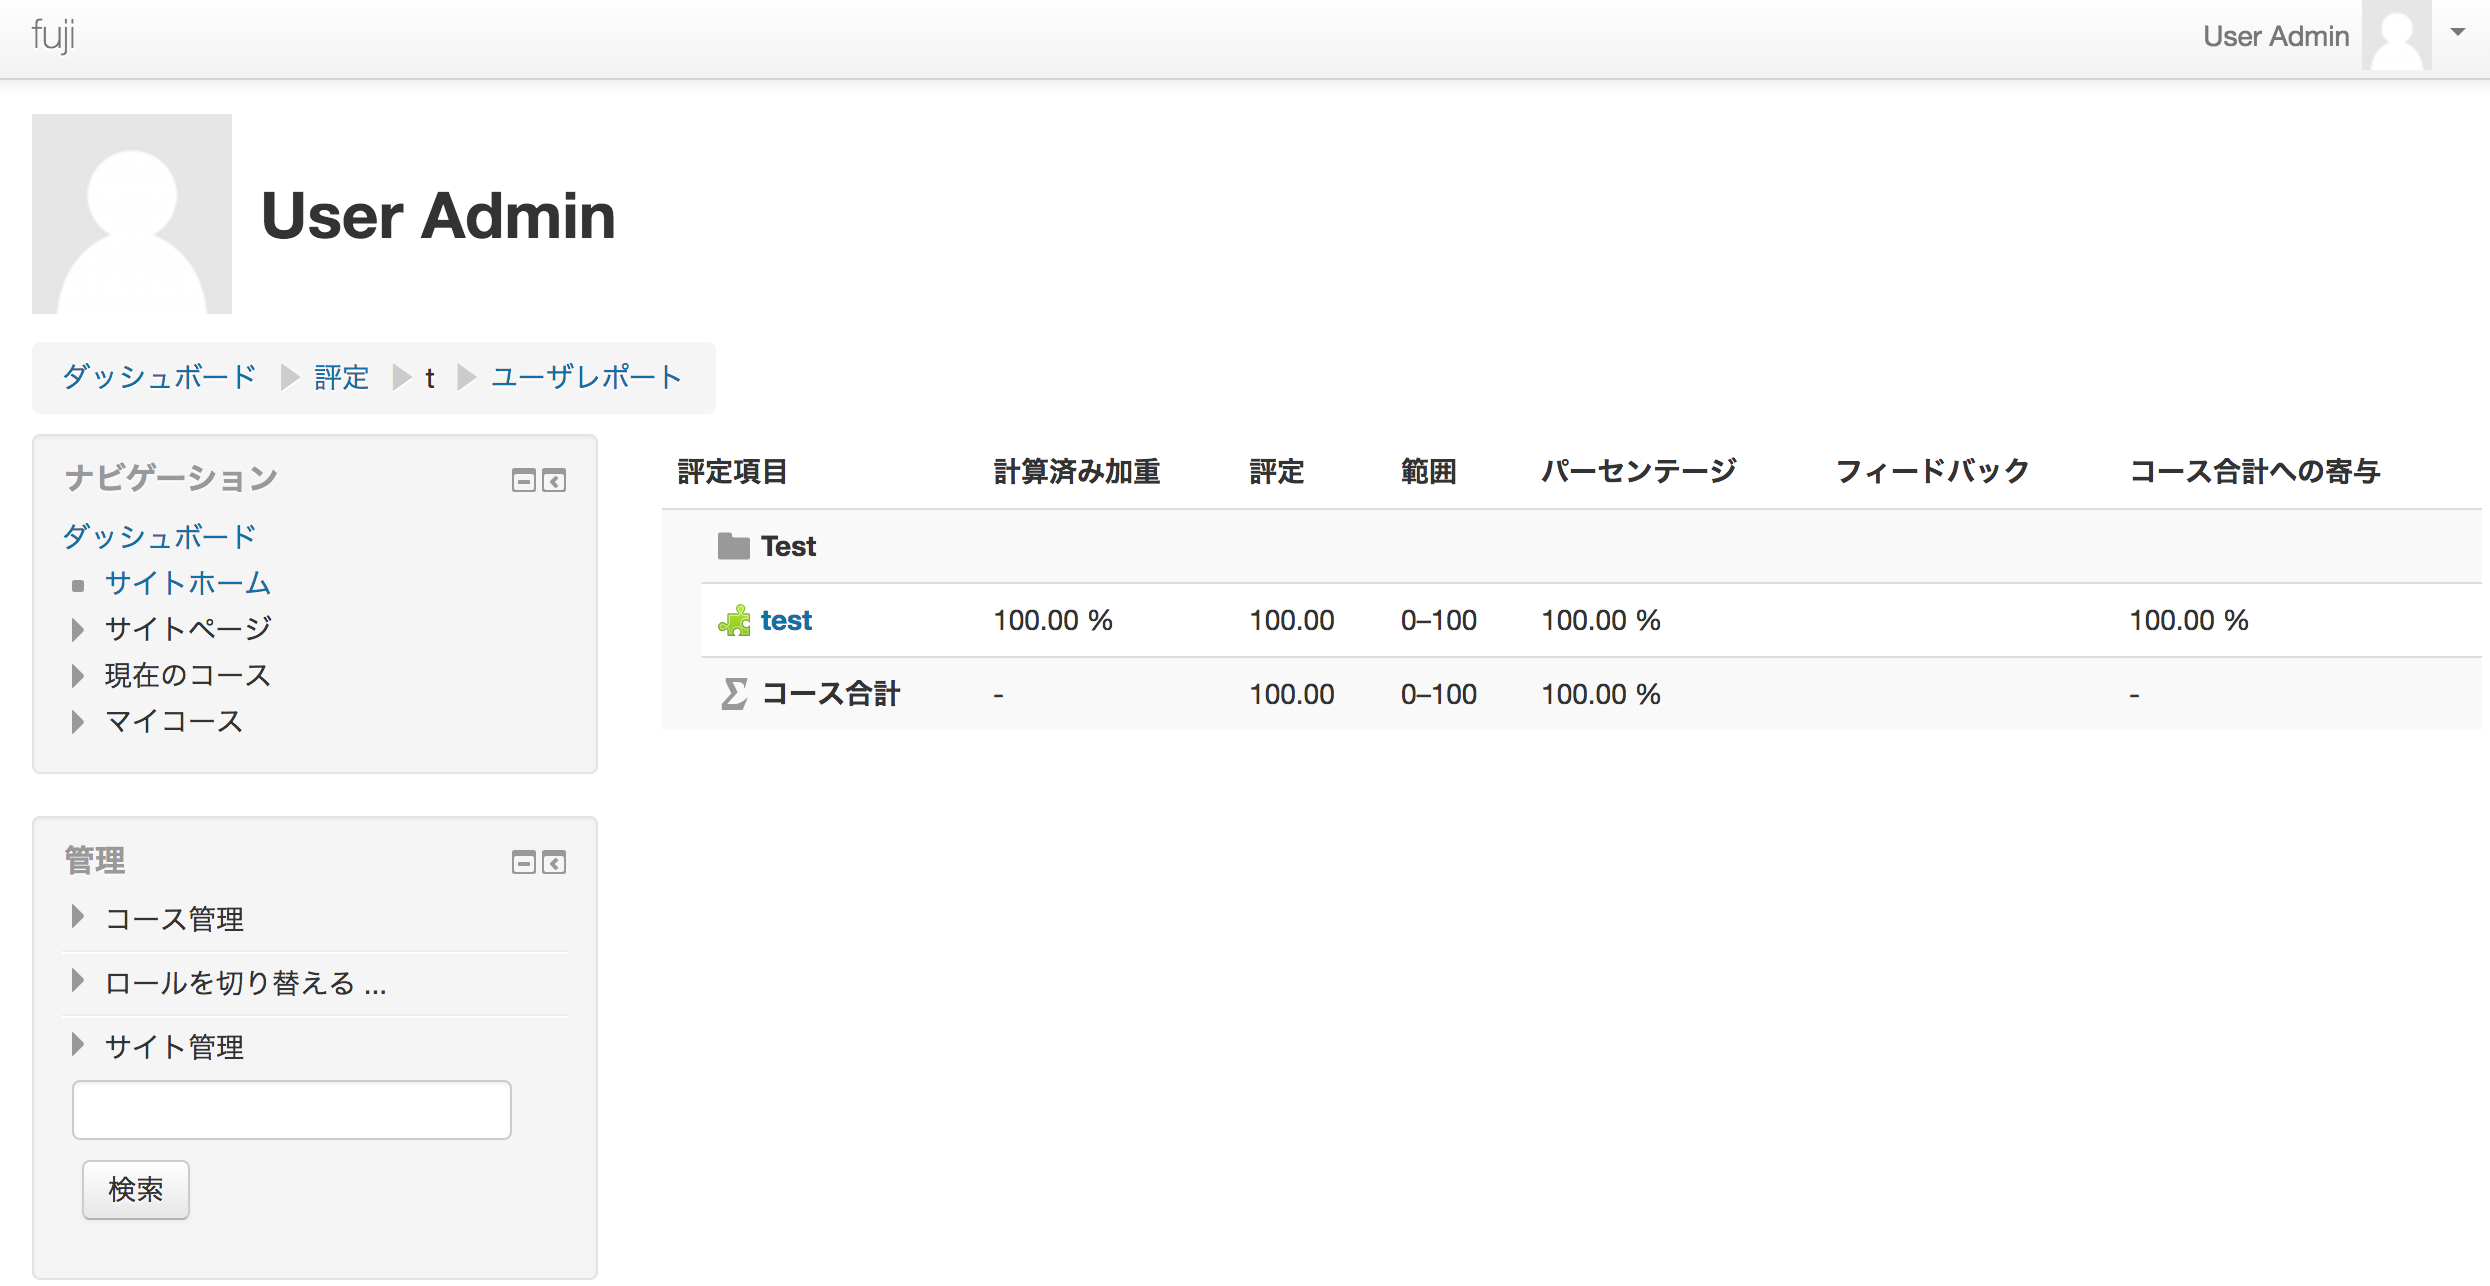
\includegraphics[clip,width=12.0cm,height=8.0cm]{img/score.png}
    \caption{moodle 成績反映}
    \label{fig:moodle score}
  \end{center}
\end{figure}
